\subsection{Erfassung und Verarbeitung von Messwerten}

\begin{wrapfigure}{R}{0.45\textwidth}
  % \begin{figure}[h]
   \vspace{-\baselineskip}
       \centering
       \includegraphics[scale=0.04]{Pictures/sensor_pflanze.jpg}
       \caption{\textit{Pflanze mit Sensor}}
       \label{img:PflanzeSensor}
  % \end{figure}
\end{wrapfigure} 

Im Praxisbeispiel sollen die erklärten Technologien Anwendung finden. Es wird ein kapazitiver Sensor verwendet,
um die Feuchtigkeit des Erdreiches zu messen. Die ermittelten Messwerte sollen per \acs{UART} vom STM32
an den ESP8266 übertragen werden.
Anschließend werden die Messwerte dem übergeordneten Netzwerk per \acs{MQTT} zur Verfügung gestellt.

\smallskip

Um präzise Messungen vorzunehmen, muss der Sensor kalibriert werden. Die Messwerte, die durch den \acs{ADC}
gemessen werden, müssen zudem in Prozent umgewandelt werden, da reine Spannungspegel wenig aussagekräftig sind.

\smallskip

Der Sensor muss während des Betriebs in das Erdreich gesteckt werden, zu sehen in Abb.\ref{img:PflanzeSensor}.




\subsubsection{Kapazitive Feuchtigkeitsmessung}

Der genutzte Sensor \citep{Sensor}, gibt die gemessene Feuchtigkeit als eine Spannung zwischen 0V und 3V aus und wird mit einer Spannung von 3.3V betrieben. Die Spannung 
entspricht demselben Spannungspegel, mit welchem auch die beiden \acs{uC} betrieben werden. Dies vereinfacht die Verwendung.

\smallskip

\begin{wrapfigure}{R}{0.45\textwidth}
  % \begin{figure}[h]
   \vspace{-\baselineskip}
       \centering
       \includegraphics[scale=0.2]{Pictures/sensor.jpg}
       \caption{\textit{Kapazitiver Sensor}}
       \label{img:Sensor}
  % \end{figure}
\end{wrapfigure}

Verbunden wird der Sensor mit dem Anschluss PA1 des STM32, welcher wiederum prozessorseitig mit dem \ac{ADC} verbunden ist \citep{STM32_Datasheet}. Auf der Platine führt
dieser Anschluss zu Pin 15 \citep{IoTGateway}. Des Weiteren sind Verbindungen zur Versorgungsspannung und dem Massepotential erforderlich \citep{Sensor}.



\subsubsection{Analog-Digital Converter}

Es wird ein einzelner Kanal des ADC1 des STM32s verwendet. Dieser wird so konfiguriert, dass eine einzelne Konversion durch Software ausgeführt wird und bei Abschluss
dieser ein Interrupt ausgelöst wird \citep{STM32_Ref}. Die Konfiguration geschieht mittels CubeMX \citep{CubeMX}.

\begin{figure}[h]
    \centering
    \begin{subfigure}{0.45\textwidth}
        \centering
        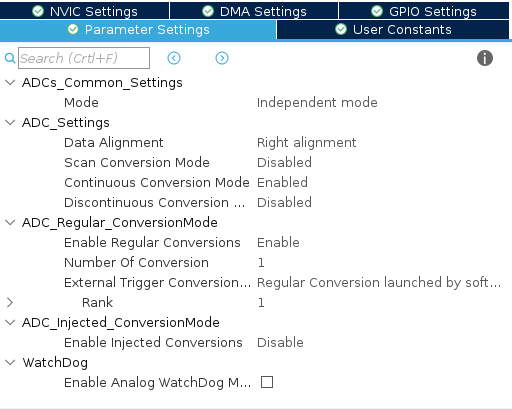
\includegraphics[width=\textwidth]{Pictures/adc_param.png}
        \caption{Parameter ADC}
        \label{img: Parameter ADC}
    \end{subfigure}
    %
    \begin{subfigure}{0.45\textwidth}
        \centering
        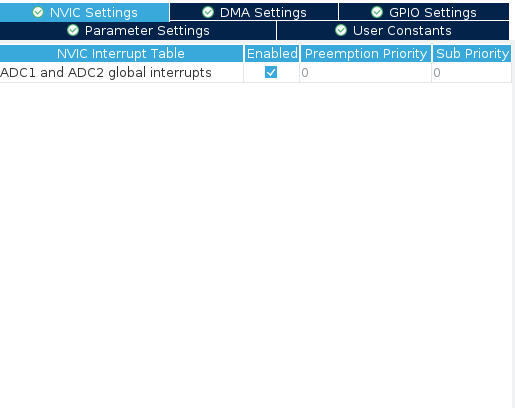
\includegraphics[width=\textwidth]{Pictures/adc_nvic.png}
        \caption{ADC Interrupt}
        \label{img: ADC Interrupt}
    \end{subfigure}
    \caption{\textit{Konfiguration des \acp{ADC}}}
    \label{img: ADC config}
  \end{figure}

  Der \ac{ADC} verfügt über eine Funktion zur Selbstkalibration \citep{STM32_Ref}. Diese wird während der Initialisierung des \ac{uC} durch folgende Funktion ausgeführt \citep{HAL_Description}:
  \begin{lstlisting}[caption={\textit{ADC Kalibrierung}}]
    HAL_ADCEx_Calibration_Start(&hadcx);      
  \end{lstlisting}

  \newpage

  Die Verarbeitung des  Interrupts des \ac{ADC} wird ähnlich realisiert, wie in \ref{subsub: Empfang} für den \ac{UART} beschrieben. Nach dem Auftreten eines 
  Interrupts wird dieser in der Routine
  \begin{lstlisting}[caption={\textit{ADC Callback}}]
    void HAL_ADC_ConvCpltCallback(ADC_HandleTypeDef *hadc)
  \end{lstlisting}  
  verarbeitet. 

  \smallskip

  Die Konversion wird mittels der Funktion \lstinline!HAL_ADC_Start_IT(&hadcx)! gestartet und kann durch \lstinline!HAL_ADC_Stop_IT(&hadcx)! gestoppt werden.

  \subsubsection{Strukturvariable SENS\_STRUCT}
  \label{subsub: SENSSTRUCT}
  Aus Gründen der Übersichtlichkeit wird eine Strukturvariable mit diversen Flags und Variablen eingeführt.
  \begin{lstlisting}[caption={\textit{Sensor Strukturvariable}}]
    typedef struct
    {
        uint8_t cal_flag;						
        uint16_t dry_value;			
        uint16_t wet_value;			
        volatile uint8_t timer_flag;	
        uint16_t an_value;			
        uint8_t percentage;			
        volatile uint8_t adc_flag;	
        uint8_t send_flag;			 
    } SENS_STRUCT;
  \end{lstlisting}

  Das Flag \lstinline!cal_flag! zeigt an, dass der Sensor kalibriert wurde. Das Flag \lstinline!adc_flag! wird genutzt, um eine vollendete Konversion des \ac{ADC} anzuzeigen.
  Um die kontinuierliche Übertragung von Messwerten freizuschalten, wird \lstinline!send_flag! genutzt. \lstinline!timer_flag! speichert, ob ein Interrupt durch einen
  Timer ausgelöst wurde.

  \smallskip
  Die Variablen \lstinline!dry_value!, \lstinline!wet_value! und \lstinline!an_value! speichern Werte zur Kalibrierung sowie den aktuellen Messwert. Dessen Repräsentation
  in Prozent wird mittels der Variablen \lstinline!percentage! gespeichert.

  

  \subsubsection{Kalibrierung des Sensors}

  \begin{wrapfigure}{R}{0.45\textwidth}
    % \begin{figure}[h]
     \vspace{-\baselineskip}
         \centering
         \includegraphics[scale=0.04]{Pictures/kalibration.jpg}
         \caption{\textit{Kalibrierung des Sensors}}
         \label{img:Kalibrierung}
    % \end{figure}
  \end{wrapfigure} 
  Der Sensor muss vor Benutzung kalibriert werden, damit eine zuverlässige Messung möglich ist. Dazu muss ein Messwert erfasst werden, wenn der Sensor komplett trocken
  ist und ein Messwert, wenn der Sensor in Wasser getränkt wird (siehe Abb. \ref{img:Kalibrierung})\citep{Sensor}. 

  \smallskip

  Die Kalibrierung wird durch den Befehl CALIBRATE, beschrieben in \ref{subsub: Nachricht}, ausgelöst. Da der Sensor für die Messung der Werte in Wasser getaucht werden soll,
  muss der Nutzer durch den Prozess begleitet werden. Dies geschieht durch die Benutzung der auf der Platine aufgelöteten LED \citep{IoTGateway}, welche abhängig vom aktuellen
  Schritt aufleuchtet. 
  Folgende Funktion der Datei \lstinline!sensor.c! implementiert die Kalibrierung:
  
  \begin{lstlisting}[caption={\textit{Funktion Kalibrierung}}]
    uint8_t cal_sens(ADC_HandleTypeDef hadc, SENS_STRUCT * sens)
  \end{lstlisting}
  
  Die Funktion gibt eine '1' bei Erfolg, oder eine '0' bei Misserfolg zurück.
  
  \smallskip

  Der Ablauf lautet wie folgt:
  \begin{itemize}
      \item Starten der Kalibrierung durch CALIBRATE
      \item LED an, Sensor muss trocken sein
      \item LED aus, Wert wird gemessen
      \item LED an, Sensor muss nass sein
      \item LED aus, Wert wird gemessen 
  \end{itemize}

  Um zuverlässige Messwerte zu erhalten, werden immer 10 Messungen durchgeführt und die gemessenen Werte gemittelt. Die Messung wird exemplarisch für den Messwert des
  trockenen Sensors erklärt. Der Zähler \lstinline!cal_counter! speichert die Anzahl der Messungen. Die Variable \lstinline!dry! speichert den gemittelten Messwert.
  
  \newpage
  
  \begin{lstlisting}[caption={\textit{Kalibrationsroutine}}]
    HAL_ADC_Start_IT(&hadc);
    while(cal_counter<10)								
    {
	    if(sens->adc_flag == 1)
        {
            cal_counter ++;
            sens->an_value = hadc.Instance->DR;
            dry += sens->an_value;
            sens->adc_flag=0;
            HAL_ADC_Start_IT(&hadc);
        }
    }
    cal_counter = 0;
    dry = dry / 10;			
    sens->dry_value = dry;
  \end{lstlisting}

  Die Messung wird durch \lstinline!HAL_ADC_Start_IT(&hadc)! gestartet. Wenn die Konversion abgeschlossen ist, wird in der entsprechenden Interruptroutine das Flag 
  \lstinline!adc_flag! gesetzt. Anschließend wird der Zähler, welcher die While-Schleife der Messung steuert, inkrementiert und der aktuelle Messwert aus dem Register
  des \ac{ADC} ausgelesen. Dieser Messwert und seine folgenden werden in der Variablen \lstinline!dry! summiert. 

  \smallskip

  Nach dem Zurücksetzen des Flags wird eine erneute Konversion gestartet, bis der Zähler seinen Endwert erreicht hat. Anschließend wird der Zähler zurückgesetzt, der Messwert
  gemittelt und an die Strukturvariable übergeben.

  \smallskip

  Die LED für die Benutzerinformation wird durch einen Timer (siehe \ref{subsub: Timer}), genauer TIM2, mit einer Periodendauer von 0.5s gesteuert. Der Timer wird mit
  der Funktion \lstinline!HAL_TIM_Base_Start_IT(&htimx)! gestartet \citep{HAL_Description}. In seiner Interruptroutine wird das Flag \lstinline!timer_flag! gesetzt. 
  \begin{lstlisting}[caption={\textit{LED Timer}}]
    HAL_TIM_Base_Start_IT(&htim2);								 
    while(sens->timer_flag)
    {
        HAL_GPIO_WritePin(LED_GPIO_Port, LED_Pin, GPIO_PIN_SET);
    }
    sens->timer_flag = 0; 												
    HAL_GPIO_WritePin(LED_GPIO_Port, LED_Pin, GPIO_PIN_RESET);
  \end{lstlisting} 
  Während das Abbruchkriterium der While-Schleife nicht erfüllt ist, wird gewartet und die LED angeschaltet. Wird der entsprechende Interrupt ausgelöst und das Flag gesetzt, führt dies 
  zum Verlassen der Schleife. Sobald die Schleife verlassen wurde, wird das Flag rückgesetzt und die LED wieder abgeschaltet.

  \smallskip

  Innerhalb der Interruptroutine wird der Timer wieder gestoppt, um ein ständiges Auslösen des Interrupts zu vermeiden.

  \smallskip

  Mit den gemessenen Werten für den feuchten und den trockenen Sensor kann nun geprüft werden, ob die Ergebnisse realistisch sind. Es ist 
  davon auszugehen, dass die Kalibration erfolgreich war, wenn der Messwert des trockenen Sensors höher ist, als der des feuchten Sensors. 
  Dies wird am Ende der Funktion geprüft und abhängig davon der Rückgabewert ausgegeben.

  \begin{lstlisting}[caption={\textit{Prüfung Ergebnisse}}]
    if((dry-wet)>0){
      return 1;										
    }
    else{
      return 0;											
    }
  \end{lstlisting}

  Der Rückgabewert wird in der Variablen \lstinline!cal_flag! des Structs \lstinline!SENS_STRUCT! gespeichert.
  

  \newpage

  \subsubsection{Berechnung des Messwertes}
  \label{subsub: Messwert}
  Mittels der durch die Kalibrierung ermittelten Werte lässt sich nun der eigentliche Messwert auf einer Skala von 0\% bis
  100\% darstellen. Die Variable \(x\) steht für den aktuellen Messwert, während \(x_{wet}\) und \(x_{dry}\) für die jeweiligen Kalibrationswerte stehen. 

  \smallskip 

  Die Formel, welche den Zusammenhang darstellt, lautet:
  \smallskip
  \begin{center}
    
  \begin{math}
        f(x)=100-\frac{(x-x_{wet})*100}{x_{wet}-x_{dry}}
  \end{math}
  \end{center}
  
  Bei der Implementation dieser Funktion in C ist bei der Nutzung von Integervariablen ohne Vorzeichen darauf zu achten, dass der Nenner nicht negativ oder 0 wird,
  da dies zu unerwartete Ergebnissen führen kann.

  \smallskip

  Die Funktion \lstinline!uint8_t val_sens(ADC_HandleTypeDef hadc, SENS_STRUCT * sens)! implementiert die Berechnung und ist in Datei \lstinline!sensor.c! zu finden.
  Um unerwarteten Ergebnisse zu vermeiden, wird geprüft, ob die Differenz zwischen den Kalibrierungswerten nicht negativ ist. Als Rückgabewert wird die 
  gemessene Feuchtigkeit in Prozent ausgegeben.

  \begin{lstlisting}[caption={\textit{Berechnung des Messwerts}}]
    uint8_t val_sens(ADC_HandleTypeDef hadc, SENS_STRUCT * sens)
    {
        uint8_t percentage;
        sens->an_value = HAL_ADC_GetValue(&hadc);
        if(sens->an_value-sens->wet_value > 0)										
        {
            percentage = 100-((sens->wet_value-sens->an_value)*100)
            /(sens->wet_value-sens->dry_value);
        }
        else
        {
            percentage = 0;
        }
        return percentage;
    }
  \end{lstlisting}

\newpage

\subsubsection{Periodisches Versenden der Messwerte}

Wurde der Sensor erfolgreich kalibriert, kann mit dem Befehl SEND\_VAL der periodische Versand der Messwerte beginnen. Wenn der Sensor nicht
kalibriert ist, wird eine Fehlermeldung versendet.

\begin{lstlisting}[caption={\textit{Periodisches Versenden von Messwerten}}]
  if(sensor.cal_flag == 1){
    HAL_TIM_Base_Start_IT(&htim1);
  }
  else{
    TxLen = er_send(ER_NOT_CAL,TxBuffer);
    HAL_UART_Transmit_DMA(&huart3, TxBuffer, TxLen);
    tx_wait(&dma_info);
  }
\end{lstlisting}

Ist der Sensor kalibriert, wird der Timer 1 (siehe \ref{subsub: Timer}) gestartet, welcher anschließend mit einer Periodendauer von 0.5s den Timer-Interrupt
auslöst. Innerhalb der Interruptroutine wird die Konversion des \ac{ADC} gestartet.
\begin{lstlisting}[caption={\textit{ADC Start}}]
	if(htim->Instance == TIM1){
		HAL_ADC_Start_IT(&hadc1);
	}  
\end{lstlisting}

Wenn dieser mit der Konversion des analogen Messwertes fertig ist, wird das entsprechende Flag \lstinline!adc_flag! der Strukturvariablen \lstinline{SENS_STRUCT} 
gesetzt (siehe \ref{subsub: SENSSTRUCT}).

\smallskip

Innerhalb der Main-Schleife wird ständig geprüft, ob dieses Flag gesetzt wurde und gegebenenfalls der Messwert in einen Prozentwert (siehe \ref{subsub: Messwert}) umgerechnet,
um anschließend versendet zu werden. Auch hier ist darauf zu achten, das Flag des \ac{ADC} \lstinline!adc_flag! wieder zurückzusetzen. Damit kein fehlerhafter Wert
versendet werden kann, wird auch geprüft, ob der Sensor kalibriert ist. Ist dies nicht der Fall, wird eine Fehlermeldung versendet (siehe \ref{list:Messwert}).

\newpage

\begin{lstlisting}[caption={\textit{Versenden Messwert}},label={list:Messwert}]
  if(sensor.adc_flag == 1)
  {
    if (sensor.cal_flag == 1)
    {
      sensor.percentage = val_sens(hadc1, &sensor);
      sensor.adc_flag = 0;
      TxLen = an_send(sensor.percentage, TxBuffer);
      HAL_UART_Transmit_DMA(&huart3, TxBuffer, TxLen);
      tx_wait(&dma_info);
    }
    else
    {
      TxLen = er_send(ER_CAL,TxBuffer);
      HAL_UART_Transmit_DMA(&huart3, TxBuffer, TxLen);
      tx_wait(&dma_info);
    }
\end{lstlisting}